\begin{center}
\begin{tikzpicture}
\node (original) at (1, 6) 
	{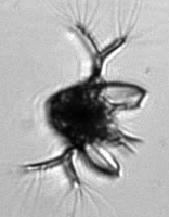
\includegraphics[width=.15\textwidth]{images/original.png}};
\node (segmented) at (5, 6)
	{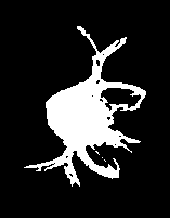
\includegraphics[width=.15\textwidth]{images/segmented.png}};
	
\node (circled) at (0, 3)
	{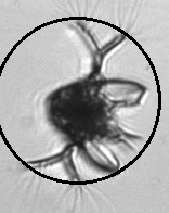
\includegraphics[width=.15\textwidth]{images/circled.png}};
\node (rected) at (3, 3)
	{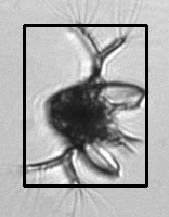
\includegraphics[width=.15\textwidth]{images/rected.png}};
\node (ellipsed) at (6, 3)
	{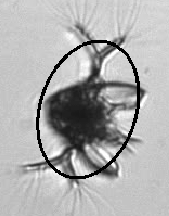
\includegraphics[width=.15\textwidth]{images/ellipsed.png}};
	
\draw[->, thick] (original.east) -- (segmented.west);
\draw[->, thick] (segmented.south) -- (circled.north);
\draw[->, thick] (segmented.south) -- (rected.north);
\draw[->, thick] (segmented.south) -- (ellipsed.north);
\draw[->, thick] (circled.south) -- (0.5, 0.7);
\draw[->, thick] (rected.south) -- (3, 0.7);
\draw[->, thick] (ellipsed.south) -- (5.5, 0.7);

\foreach \i in {0,...,12}
{
	\pgfkeys{/pgf/number format/.cd,fixed,precision=0}
	\pgfmathsetmacro\myvalue{abs(rand) * 10}
	\draw[fill=blue!45!white] (0.5 * \i, 0) rectangle (0.5 + 0.5 * \i, 0.5) node[pos=.5]{\pgfmathprintnumber\myvalue};
}
\end{tikzpicture}
\end{center}